\documentclass[12pt,a4paper]{article}

% ─── Page Layout ───────────────────────────────────────────────────────────────
\usepackage[a4paper, margin=0.8in, headheight=14pt]{geometry}

% ─── Fonts (XeLaTeX) ───────────────────────────────────────────────────────────
\usepackage{fontspec}
\usepackage{unicode-math}
\setmainfont{TeX Gyre Pagella}
\setmonofont[Scale=0.88]{TeX Gyre Cursor}
\setmathfont{Latin Modern Math}

% ─── Packages ──────────────────────────────────────────────────────────────────
\usepackage{xcolor}
\usepackage{colortbl}
\usepackage{titlesec}
\usepackage{enumitem}
\usepackage{tabularx}
\usepackage{booktabs}
\usepackage{array}
\usepackage{amsmath}
\usepackage{tikz}
\usetikzlibrary{shapes.geometric, arrows.meta, positioning, calc, fit, decorations.pathreplacing}
\usepackage{tcolorbox}
\tcbuselibrary{skins, breakable}
\usepackage{hyperref}
\usepackage{fancyhdr}
\usepackage{graphicx}
\usepackage{microtype}
\hyphenpenalty=10000
\exhyphenpenalty=10000
\sloppy
\usepackage{caption}
\usepackage{setspace}
\usepackage{multirow}
\usepackage{tocloft}

% ─── Q&A helper ────────────────────────────────────────────────────────────────
\newcommand{\Q}[1]{\textbf{#1}\par\noindent\ignorespaces}

% ─── Colour Palette ────────────────────────────────────────────────────────────
\definecolor{myred}{RGB}{196,30,58}
\definecolor{mydark}{RGB}{30,30,50}
\definecolor{mygreen}{RGB}{14,120,80}
\definecolor{myteal}{RGB}{0,130,140}
\definecolor{myamber}{RGB}{180,100,0}
\definecolor{mypurple}{RGB}{100,30,160}
\definecolor{mygray}{RGB}{246,247,249}
\definecolor{mgframe}{RGB}{180,185,200}
\definecolor{watermark}{RGB}{145,150,170}
\definecolor{hdrred}{RGB}{250,232,235}
\definecolor{hdrgreen}{RGB}{220,244,233}
\definecolor{hdrteal}{RGB}{220,242,244}
\definecolor{hdramber}{RGB}{253,242,215}
\definecolor{hdrpurple}{RGB}{238,228,255}
\definecolor{hdrgray}{RGB}{238,240,245}
\definecolor{rowalt}{RGB}{250,251,253}

% ─── Section Formatting ────────────────────────────────────────────────────────
\titleformat{\section}
  {\large\bfseries\color{myred}}{\thesection.}{0.5em}{}
  [\vspace{1pt}{\color{myred}\rule{\linewidth}{0.8pt}}]
\titleformat{\subsection}
  {\normalsize\bfseries\color{myteal}}{\thesubsection}{0.5em}{}
\titlespacing*{\section}{0pt}{18pt}{7pt}
\titlespacing*{\subsection}{0pt}{11pt}{4pt}

% ─── Paragraph ─────────────────────────────────────────────────────────────────
\setlength{\parindent}{0pt}
\setlength{\parskip}{4pt}

% ─── TOC Styling ───────────────────────────────────────────────────────────────
\renewcommand{\cfttoctitlefont}{\large\bfseries\color{myred}}
\renewcommand{\cftaftertoctitle}{\par\noindent{\color{myred}\rule{\linewidth}{0.8pt}}}
\setlength{\cftbeforetoctitleskip}{0pt}
\setlength{\cftaftertoctitleskip}{6pt}
\renewcommand{\cftsecfont}{\normalsize\bfseries\color{mydark}}
\renewcommand{\cftsecpagefont}{\normalsize\bfseries\color{mydark}}
\renewcommand{\cftsecleader}{\cftdotfill{\cftdotsep}}
\setlength{\cftbeforesecskip}{7pt}
\renewcommand{\cftsubsecfont}{\small\color{mydark}}
\renewcommand{\cftsubsecpagefont}{\small\color{mydark}}
\setlength{\cftbeforesubsecskip}{3pt}
\setlength{\cftsubsecindent}{1.4em}

% ─── Table helpers ─────────────────────────────────────────────────────────────
\renewcommand{\arraystretch}{1.45}
\setlength{\tabcolsep}{6pt}
\arrayrulecolor{mydark}
\newcolumntype{B}[1]{>{\small\bfseries\raggedright\arraybackslash}m{#1}}
\newcolumntype{Y}{>{\small\raggedright\arraybackslash}X}
\renewcommand{\tabularxcolumn}[1]{m{#1}}

% ─── Header / Footer ───────────────────────────────────────────────────────────
\pagestyle{fancy}
\fancyhf{}
\fancyhead[L]{\small\color{myred}\textbf{EC502}\;\color{mydark}--- Computer Architecture}
\fancyhead[R]{\small\color{myteal}\textbf{Module 2 Notes}}
\fancyfoot[C]{\small\color{mydark}\thepage}
\fancyfoot[R]{\small\color{watermark}\textit{\copyright\ Biraj}}
\renewcommand{\headrulewidth}{0.5pt}
\renewcommand{\footrulewidth}{0.3pt}

% ─── Hyperref ──────────────────────────────────────────────────────────────────
\hypersetup{
  colorlinks=true, linkcolor=myteal, urlcolor=myteal,
  pdfauthor={Biraj Sarkar},
  pdftitle={EC502 --- Module 2 Notes}
}

% ─── tcolorbox styles ──────────────────────────────────────────────────────────
\tcbset{
  tikzbox/.style={
    colback=mygray, colframe=mgframe, boxrule=0.6pt, arc=4pt,
    left=8pt, right=8pt, top=6pt, bottom=6pt,
    colbacktitle=mgframe, coltitle=mydark,
    fonttitle=\small\bfseries
  },
  defbox/.style={
    colback=hdrgreen, colframe=mygreen, boxrule=0.8pt, arc=4pt,
    left=9pt, right=9pt, top=6pt, bottom=6pt,
    colbacktitle=mygreen, coltitle=white,
    fonttitle=\small\bfseries
  },
  formulabox/.style={
    colback=hdrteal, colframe=myteal, boxrule=0.8pt, arc=4pt,
    left=9pt, right=9pt, top=7pt, bottom=7pt,
    colbacktitle=myteal, coltitle=white,
    fonttitle=\small\bfseries
  },
  examplebox/.style={
    colback=hdramber, colframe=myamber, boxrule=0.8pt, arc=4pt,
    left=9pt, right=9pt, top=6pt, bottom=6pt,
    colbacktitle=myamber, coltitle=white,
    fonttitle=\small\bfseries
  },
  masonbox/.style={
    colback=hdrpurple, colframe=mypurple, boxrule=0.8pt, arc=4pt,
    left=9pt, right=9pt, top=6pt, bottom=6pt,
    colbacktitle=mypurple, coltitle=white,
    fonttitle=\small\bfseries
  },
  exambox/.style={
    colback=hdrpurple, colframe=mypurple, boxrule=1pt, arc=5pt,
    left=10pt, right=10pt, top=8pt, bottom=8pt,
    colbacktitle=mypurple, coltitle=white,
    fonttitle=\bfseries,
    breakable, title after break={\textbf{Frequently Asked / Viva Questions (contd.)}}}
}
% Make all boxes breakable across pages
\tcbset{breakable}

% ─── TikZ styles ───────────────────────────────────────────────────────────────
\tikzset{
  block/.style={rectangle, draw=myteal, fill=hdrteal,
    text width=2.4cm, align=center, minimum height=0.95cm,
    font=\small, rounded corners=3pt, line width=0.7pt},
  redblock/.style={rectangle, draw=myred, fill=hdrred,
    text width=2.4cm, align=center, minimum height=0.95cm,
    font=\small, rounded corners=3pt, line width=0.7pt},
  netnode/.style={rectangle, draw=myteal, fill=hdrteal,
    text width=1.5cm, align=center, minimum height=0.8cm,
    font=\small, rounded corners=3pt, line width=0.7pt},
  sumjunc/.style={circle, draw=myamber, fill=hdramber,
    minimum size=0.62cm, font=\small, line width=0.8pt},
  snode/.style={circle, draw=mypurple, fill=hdrpurple,
    minimum size=0.55cm, font=\footnotesize, line width=0.7pt},
  arrow/.style={-Stealth, thick, color=mydark},
  redarrow/.style={-Stealth, thick, color=myred},
  line/.style={thick, color=mydark}
}

% ═══════════════════════════════════════════════════════════════════════════════
\begin{document}
% ═══════════════════════════════════════════════════════════════════════════════

\begin{center}
  {\LARGE\bfseries\color{myred} EC502 --- Computer Architecture}\\[5pt]
  {\normalsize\color{mydark} Semester V \quad$\bullet$\quad 3L:0T:0P \quad$\bullet$\quad 3 Credits}\\[3pt]
  {\normalsize\color{myteal}\textbf{Module 2 Exam Notes: Processor Organisation and Data Representation}}\\[3pt]
  {\small\color{mydark} CGEC \;$|$\; B.Tech ECE (2023--27) \;$|$\; \textit{Biraj Sarkar}}
\end{center}
\vspace{2pt}
\noindent{\color{myred}\rule{\linewidth}{1.5pt}}
\vspace{2pt}

\hypersetup{linkcolor=mydark}
\tableofcontents
\hypersetup{linkcolor=myteal}
\newpage

\section{Processor Organisation and Data Representation}
\begin{tcolorbox}[defbox,title={Datapath and register-transfer language}]
A datapath is the collection of registers, buses, multiplexers and functional units that hold and transform data. Register-transfer language (RTL) describes operations such as $R_3\leftarrow R_1+R_2$ and the clock events at which registers update.
\end{tcolorbox}
\subsection{Registers, bus structure and flags}
\begin{itemize}[leftmargin=*,itemsep=3pt]
\item \textbf{PC and IR.} The program counter supplies the next instruction address. The instruction register (IR) holds the instruction being decoded or executed in a simple CPU.
\item \textbf{MAR and MDR.} The memory address register (MAR) drives an address. The memory data register (MDR), also called MBR in some models, buffers memory data. In practice these roles may be part of a memory interface rather than named registers.
\item \textbf{General registers and status.} General-purpose registers hold operands and addresses. An accumulator is an implicit operand/result register in an accumulator organisation. Typical status flags are zero $Z$, negative $N$, carry $C$ and signed overflow $V$.
\item \textbf{Internal bus.} On a single bus, select one source driver at a time. Multiple destination registers may latch the same value together. Multiport register files and multiple buses can carry separate inputs and a result in one cycle.
\end{itemize}
\begin{tcolorbox}[tikzbox,title={A three-bus register datapath},unbreakable]
\centering
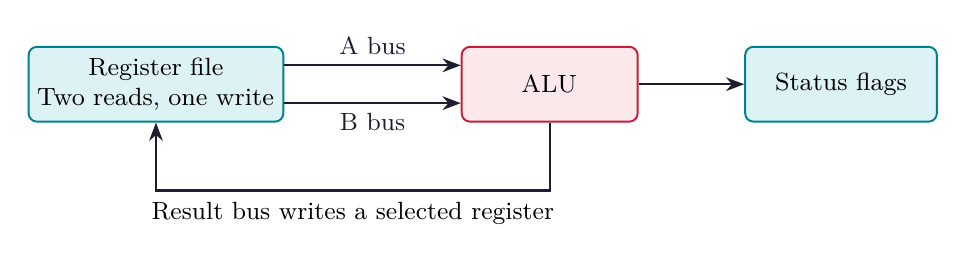
\begin{tikzpicture}[font=\small]
\node[block,text width=3cm] (rf) at (0,0) {Register file\\Two reads, one write};
\node[redblock,text width=2cm] (alu) at (5,0) {ALU};
\node[block,text width=2.2cm] (flags) at (8.7,0) {Status flags};
\draw[arrow] ($(rf.east)+(0,.24)$)--($(alu.west)+(0,.24)$) node[midway,above] {A bus};
\draw[arrow] ($(rf.east)+(0,-.24)$)--($(alu.west)+(0,-.24)$) node[midway,below] {B bus};
\draw[arrow] (alu.east)--(flags.west);
\draw[arrow] (alu.south)--(5,-1.35)--(0,-1.35)--(rf.south);
\node[below] at (2.5,-1.37) {Result bus writes a selected register};
\end{tikzpicture}
\end{tcolorbox}

\begin{tcolorbox}[examplebox,title={One-bus versus three-bus addition}]
For $R_3\leftarrow R_1+R_2$ on a single bus, use temporary registers $Y$ and $Z_{\rm ALU}$.
\begin{enumerate}[leftmargin=*,itemsep=2pt]
\item Place $R_1$ on the bus and latch it in $Y$.
\item Place $R_2$ on the bus, select ADD and latch $Y+R_2$ in $Z_{\rm ALU}$.
\item Place $Z_{\rm ALU}$ on the bus and write $R_3$.
\end{enumerate}
In the illustrated three-bus model, $R_1$ and $R_2$ can be read simultaneously and the result can be written at the clock edge, if the combinational path meets timing.
\end{tcolorbox}

\par\vspace{6pt}\noindent
\begin{tabularx}{\linewidth}{|B{3.2cm}|Y|Y|}\hline
Organisation & Operand and result convention & Trade-off \\ \hline
Accumulator & ALU uses an implicit accumulator and writes it back. & Compact fields, but frequent accumulator spills are possible. \\ \hline
General register & Explicit register fields select operands. & Flexible reuse of values at the cost of more encoding bits and ports. \\ \hline
Stack & ALU removes top entries and pushes one result. & Compact arithmetic encodings. Operand access and data dependence are tied to stack order. \\ \hline
\end{tabularx}

\section{Binary Information and Number Formats}
\subsection{Positional notation, characters and bytes}
\begin{tcolorbox}[defbox,title={Bit, byte and word}]
A bit represents one of two states. A byte has eight bits. A word is a machine-defined unit of data, often 16, 32 or 64 bits. The same pattern can represent an integer, character, instruction or part of an address depending on its interpretation.
\end{tcolorbox}
\begin{itemize}[leftmargin=*,itemsep=3pt]
\item \textbf{Radix.} A digit at position $i$ has weight $b^i$ in radix $b$. For base 2, $(1011.101)_2=8+2+1+1/2+1/8=11.625$.
\item \textbf{Conversion.} Repeatedly divide an integer by the target radix and read remainders in reverse. Repeatedly multiply the fraction by the radix and record each integer part in order. For instance $0.375$ becomes $0.011_2$ because successive products give digits 0, 1, 1.
\item \textbf{Octal and hexadecimal.} Group binary bits in threes for octal or fours for hex, starting at the radix point. Thus $(1101\,0110)_2=\texttt{D6}_{16}$. Pad only the outer ends when needed.
\item \textbf{Binary-coded decimal (BCD).} Encode each decimal digit in four bits. Decimal 59 is \texttt{0101 1001} in 8421 BCD but \texttt{0011 1011} as an unsigned binary integer.
\item \textbf{Character representation.} ASCII assigns codes to 128 basic symbols. Unicode assigns code points and encodings such as UTF-8 store their byte representations. For example, ASCII and UTF-8 both encode \texttt{A} as hex \texttt{41}.
\end{itemize}
\begin{tcolorbox}[examplebox,title={Identify endianness by increasing addresses}]
Store \texttt{0x12345678} as a four-byte word starting at address 100. In big-endian order, addresses 100--103 contain \texttt{12 34 56 78}. In little-endian order, they contain \texttt{78 56 34 12}. Endianness orders bytes in memory. It does not reverse the bits within a byte.
\end{tcolorbox}

\subsection{Signed integers and overflow}
\par\vspace{6pt}\noindent
\begin{tabularx}{\linewidth}{|B{3.5cm}|Y|Y|}\hline
Encoding & For $n$ bits & 8-bit example for $-13$ \\ \hline
Unsigned & $0$ to $2^n-1$. No negative values. & Not representable. \\ \hline
Sign and magnitude & A sign bit and $n-1$ magnitude bits, including two zeros. & \texttt{10001101} \\ \hline
One's complement & Invert all bits of the positive form. Two zeros. & \texttt{11110010} \\ \hline
Two's complement & Invert and add one. Range $-2^{n-1}$ to $2^{n-1}-1$. One zero. & \texttt{11110011} \\ \hline
Biased & Stored unsigned code is value plus a stated bias. & With bias 127, $114=$ \texttt{01110010}. \\ \hline
\end{tabularx}

In two's complement the top bit has weight $-2^{n-1}$. Add or subtract modulo $2^n$, discarding the carry beyond the width. Extend a signed operand by repeating its sign bit. Extend an unsigned operand with zeros. For addition, signed overflow occurs if equal-sign operands yield an opposite-sign result. Equivalently $V=C_{\rm into\ sign}\oplus C_{\rm out\ of\ sign}$. Unsigned addition overflow uses the final carry. For subtraction $A-B$ using $A+\overline B+1$, carry out 1 means no unsigned borrow under this convention.
\begin{tcolorbox}[examplebox,title={Trace signed arithmetic and test the result}]
In eight bits, $+45=\texttt{00101101}$ and $-19=\texttt{11101101}$.
\[
\begin{aligned}
(+45)+(-19)&=\texttt{00101101}+\texttt{11101101}
             =\texttt{00011010}=26,\\
(-45)-(-19)&=\texttt{11010011}+\texttt{00010011}
             =\texttt{11100110}=-26.
\end{aligned}
\]
Both results fit and the first addition's discarded carry does not indicate signed overflow. In four bits $7+3$ gives \texttt{1010}, an invalid signed sum, because two positive operands yielded a negative sign. The same bit pattern correctly encodes unsigned decimal 10.
\end{tcolorbox}

\subsection{Fixed-point and floating-point interpretation}
\begin{itemize}[leftmargin=*,itemsep=4pt]
\item \textbf{Fixed point.} Assign $F$ fractional bits to a stored integer $I$. Its value is $I2^{-F}$, with constant step $2^{-F}$. For an eight-bit signed encoding with $F=4$, range is $-8$ to $7.9375$. The pattern \texttt{11101100} is $I=-20$, hence $-1.25$.
\item \textbf{Fixed-point arithmetic.} Align binary points before addition. The raw product of two values with $F$ fractional bits has $2F$ fractional bits. For a result with $F$ fractional bits, rescale, round and test for overflow.
\item \textbf{Floating point.} Represent a value using sign, significand and an exponent, for example $-1.01_2\times2^3=-10$. Exponents give a larger dynamic range while spacing between adjacent values generally grows with magnitude.
\item \textbf{When to use each.} A known bounded scale can make fixed-point hardware simple and predictable. Floating point accommodates values of widely different sizes, but exponent alignment and rounding add work.
\end{itemize}

\newpage
\begin{center}
  {\large\bfseries\color{myred} Quick Revision --- Module 2}\\[3pt]
  {\small\color{mydark} Processor Organisation and Data Representation $|$ EC502}
\end{center}
\noindent{\color{myred}\rule{\linewidth}{1.2pt}}
\begin{tcolorbox}[formulabox,title={Key Formulas at a Glance}]
\renewcommand{\arraystretch}{1.35}
\begin{tabularx}{\linewidth}{B{5.0cm}Y}
Unsigned range & $0\le x\le 2^n-1$ \\[3pt]
Two's-complement range & $-2^{n-1}\le x\le 2^{n-1}-1$ \\[3pt]
Fixed-point value & $x=I2^{-F}$ with scale $F$ fractional bits \\[3pt]
Signed addition overflow & $V=C_{\rm into\ sign}\oplus C_{\rm out\ of\ sign}$ \\[3pt]
\end{tabularx}
\end{tcolorbox}
\begin{tcolorbox}[defbox,title={One-Line Definitions}]
\textbf{Datapath.} Hardware that stores, routes and transforms operands.\par
\textbf{Sign extension.} Increase two's-complement width by copying the sign bit into the added high positions.\par
\textbf{Endianness.} Order of bytes of a multi-byte value in memory.\par
\end{tcolorbox}
\begin{tcolorbox}[exambox,title={Frequently Asked / Viva Questions}]
\begin{enumerate}[topsep=0pt, label=\textbf{Q\arabic*.}, itemsep=5pt]
\item \Q{What does RTL describe?}
Register transfers and operations scheduled by control signals and clock events.
\item \Q{Why can a single bus not carry two unrelated inputs at once?}
It selects one value source for that transfer.
\item \Q{What is the role of MAR?}
Hold or present the memory transaction address.
\item \Q{How many zeros exist in one's complement?}
Two, the all-zero and all-one patterns.
\item \Q{How is a two's-complement negative obtained?}
Invert the bits and add one within the chosen width.
\item \Q{Can opposite-sign addition overflow in two's complement?}
No, because the integer sum is between the two operands.
\item \Q{What is the carry--borrow convention for the illustrated subtractor?}
Carry out 1 means no unsigned borrow.
\item \Q{Is BCD the same as binary coding of the whole number?}
BCD encodes each decimal digit separately.
\item \Q{Which byte comes first in little-endian memory?}
The least significant byte goes at the lowest address.
\item \Q{Why does floating-point spacing vary?}
Changing the exponent scales the spacing between adjacent significands.
\end{enumerate}
\end{tcolorbox}
\begin{tcolorbox}[tikzbox,title={Summary comparison}]
\begin{tabularx}{\linewidth}{|B{4cm}|Y|}\hline
\textbf{Case} & \textbf{What to use} \\ \hline
MAR / MDR & Address for memory / data going to or from memory. \\ \hline
Fixed point & Constant step and explicitly assigned scale. \\ \hline
Floating point & Significand and exponent trading precision and dynamic range. \\ \hline
\end{tabularx}
\end{tcolorbox}
\end{document}
